%!TEX root = batch-course.tex
%-------------------------------------------------
\section{Batch analysis using feature extraction}
%-------------------------------------------------

\begin{frame}\frametitle{Feature extraction methods: overview}

\begin{itemize}
	\item	Unaligned data can be a challenge (more later).
	
	\item	One alternative to alignment, if we want to get started right away: 
	
			\begin{itemize}
				\item	{\color{myOrange}{\emph{extract features}}} from each phase in each batch
				
				\item	assemble features within a row\pause
				
				\item	build ordinary PCA on \( \mathbf{X_f} \) or PLS: \( \left\{ \mathbf{Z} \,\,\text{and}\,\, \mathbf{X_f}\right\} \stackrel{\text{PLS}}{\longmapsto} \mathbf{Y} \)
			\end{itemize}
\end{itemize}

\begin{center}
	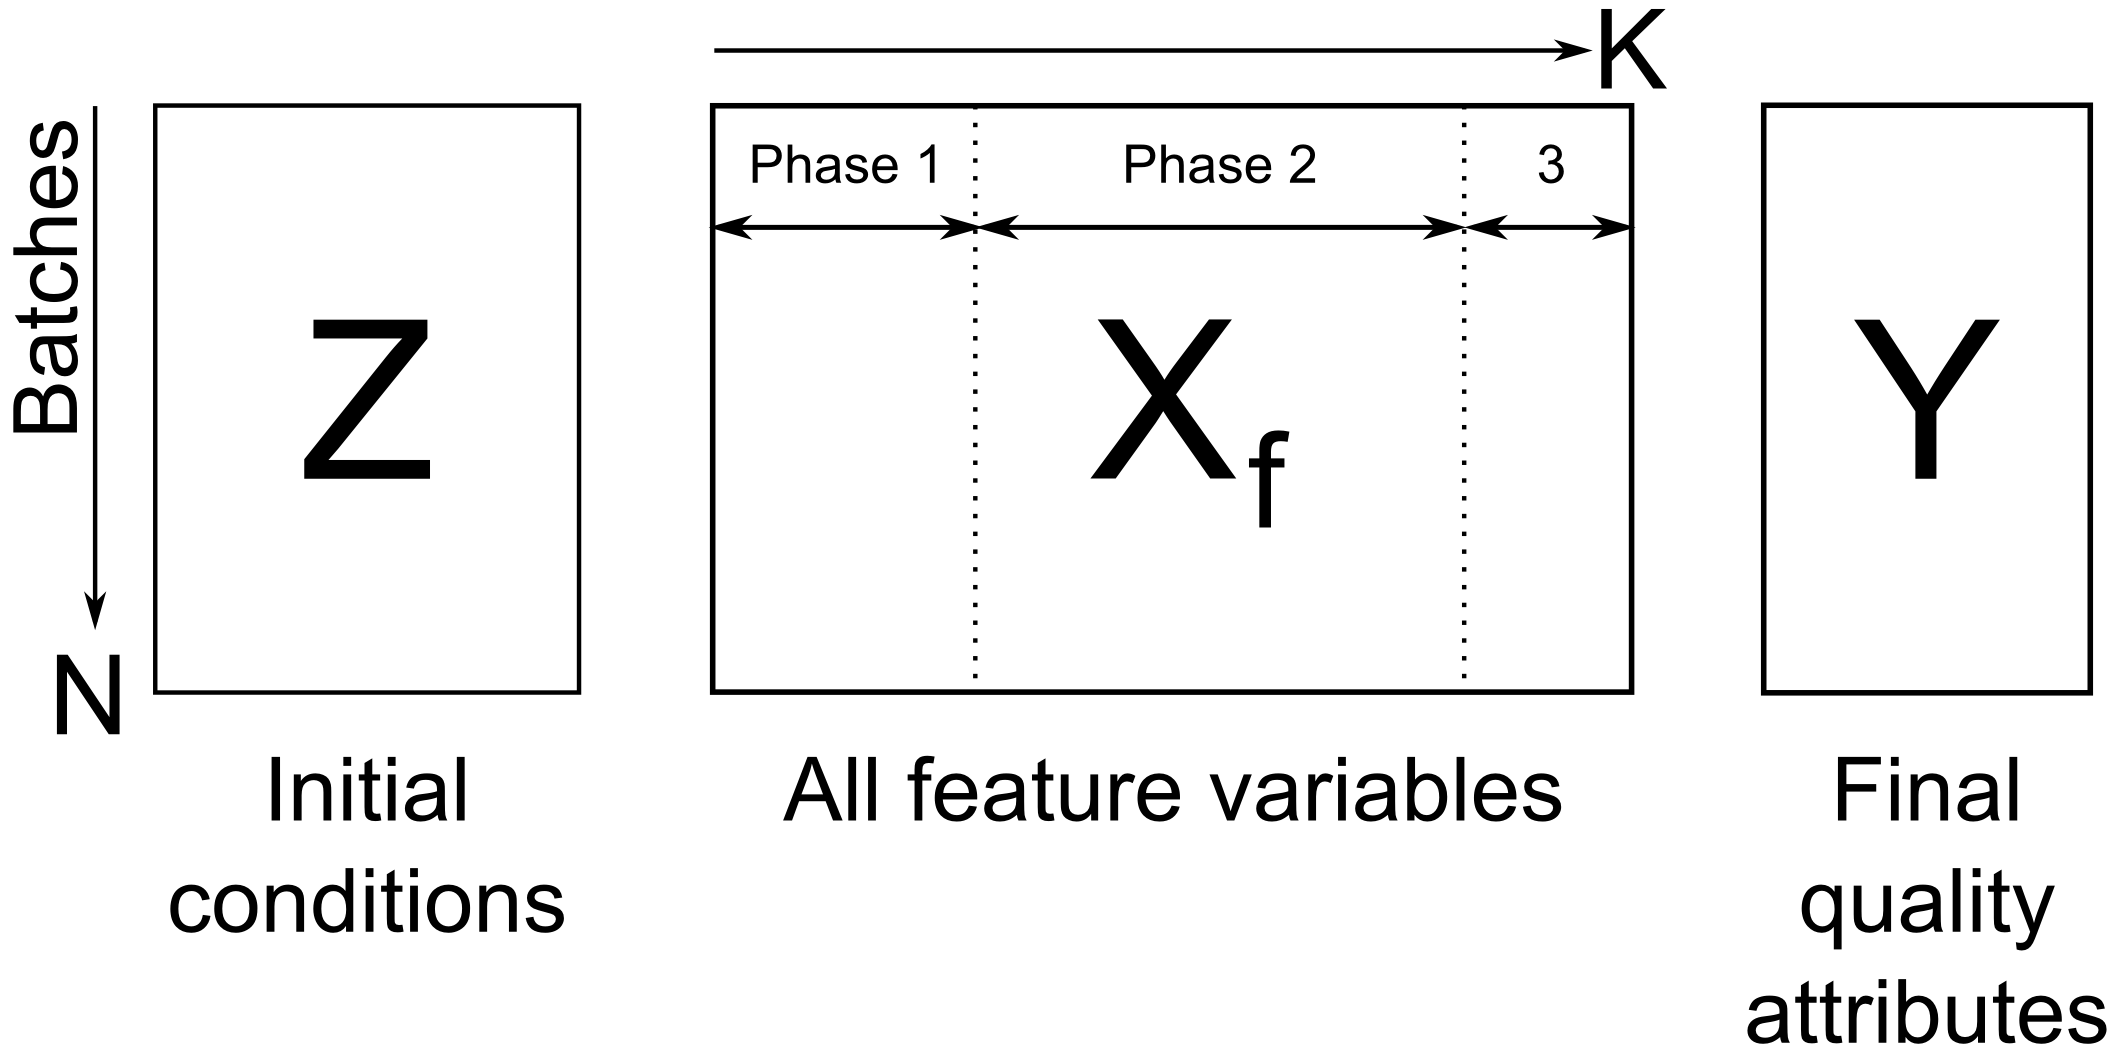
\includegraphics[width=0.95\textwidth]{images/data-after-feature-extraction.png}
\end{center}
\end{frame}

\begin{frame}\frametitle{Which features to extract}

\begin{itemize}
	\item	Extract {\color{myGreen}{\emph{within each phase}}} or within {\color{myGreen}{\emph{specified windows}}}. 
	
	\item	Extract for one, some, or \textbf{all} tags:
\end{itemize}\pause

\begin{itemize}
	\item	average value \hfill {\color{myOrange} $\leftarrow$ easiest, most useful feature}
	\item 	median value
	\item	integrated area under a tag (often makes engineering sense)
	\item	standard deviation, (useful if tag should be constant)
	\item	slope of curve\pause
	\item	energy or mass balance calculation over a phase
	 		\begin{itemize}
	 			\item	e.g. heat released by a reaction should be taken up by the cooling water
	 			\item	an imbalance can point out a problematic batch
	 		\end{itemize} \pause
	\item	value of a trajectory at start/end of phase
	\item	total time for a phase to complete (goes into \( \mathbf{Z} \))
\end{itemize}
\end{frame}

\begin{frame}\frametitle{How to use feature-based models}

\begin{itemize}
	\item	Many features extracted: often \( \sim \) 80 to 100 columns; many are not useful
	
	\item	Used in an ordinary PCA or PLS.  All the usual tools apply:
	
			\begin{itemize}
				\item	VIP: finds most import variables for explaining CQAs \( (\mathbf{Y}) \)
				
				\item	loadings and weights: used to interpret any clusters in the scores
				
				\item	use \( R^2 \) per variable and small weights to decide which on less-useful features to eliminate
			\end{itemize}\pause
	
	\item	Learn about the batch: {\small e.g.: variability in cooling water temperature related to poor CQA}
	
	\item	Troubleshooting an unusual batch 

	\item	By extension, use troubleshooting information to improve future batches \pause
	
	\item	Can be used for monitoring: we'll come back to this
\end{itemize}
\end{frame}

\begin{frame}\frametitle{Disadvantages of feature-based models}

\begin{itemize}
	\item	Smoothly varying trajectories within a phase
	
			\begin{itemize}
				\item	no distinct features and hard to quantify
			\end{itemize}

\end{itemize}

\begin{center}
	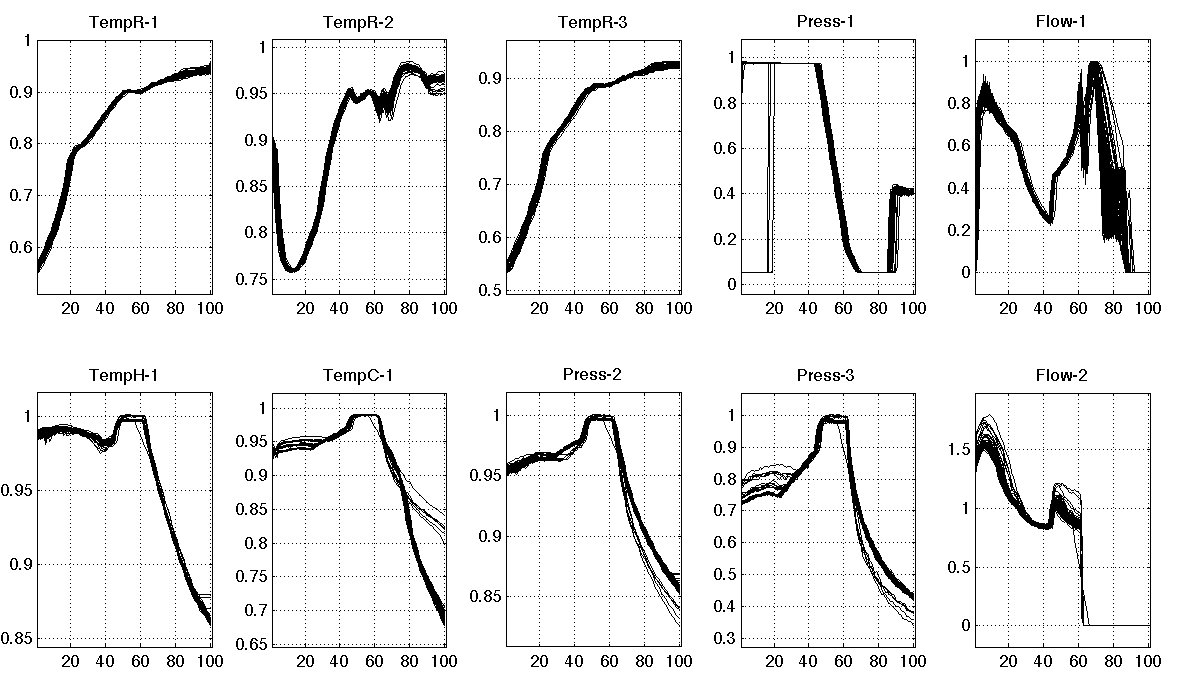
\includegraphics[width=\textwidth]{images/smooth-trajectories-unsuitable-for-features.png}
\end{center}

\end{frame}

\begin{frame}\frametitle{Disadvantages of feature-based models}

\begin{itemize}
	\item	Features to choose depend on engineer's prior knowledge
	
	\item	Subtle defects and broken correlations between variables 
	
			\begin{itemize}
				\item	hard/impossible to detect and quantify
			\end{itemize}

	\item	Feature value may not exist in an abnormal batch: so it's missed

\end{itemize}

\begin{center}
	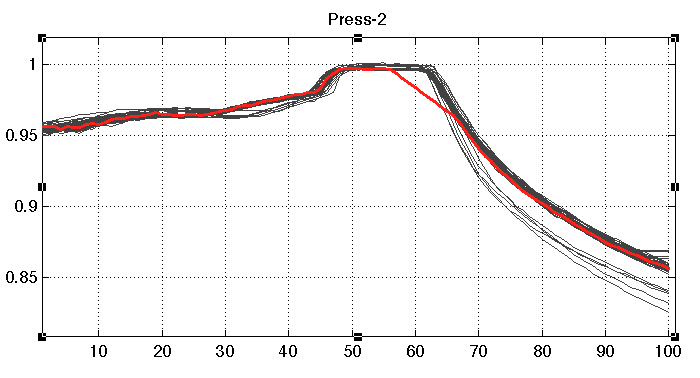
\includegraphics[width=0.9\textwidth]{images/features-subtle-problems-can-go-undetected.png}
\end{center}

\end{frame}

\begin{frame}\frametitle{Class example: using feature-based models}

	\begin{itemize}
		
		\item	Feature example for this batch process works well
		
				\begin{itemize}
				
					\item	4 distinct phases with ``sharp'' trajectories
				
				\end{itemize}

	\end{itemize}

	\begin{center}
		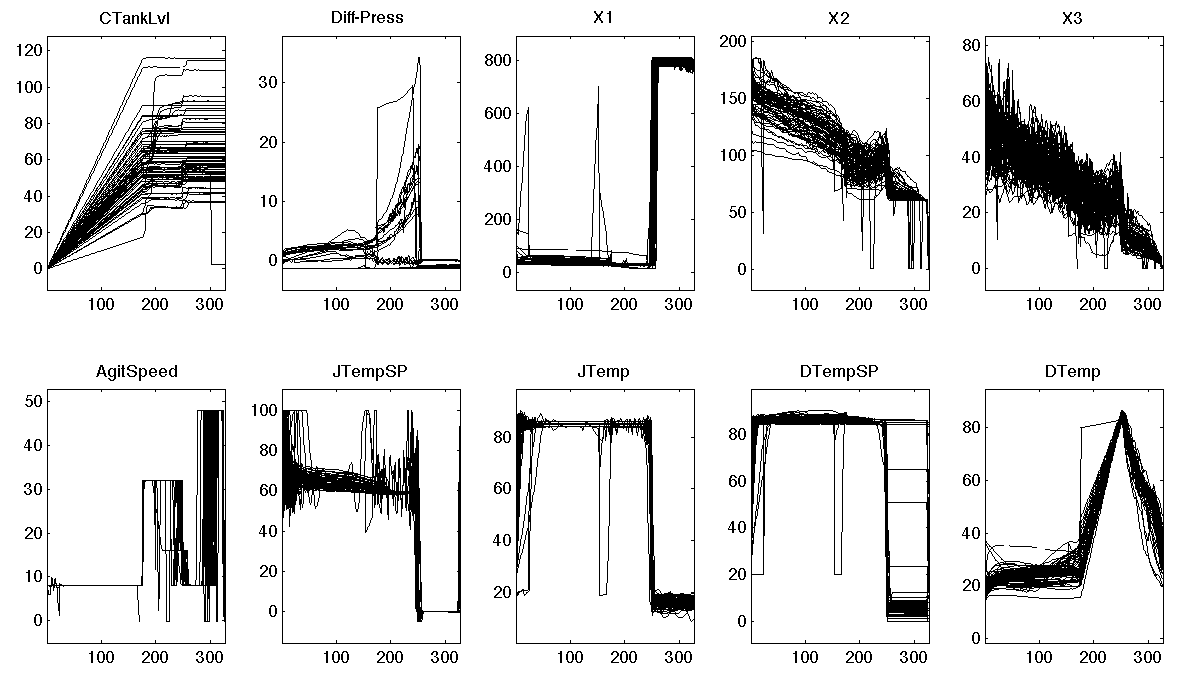
\includegraphics[width=\textwidth]{images/fmc/fmc-raw-trajectories.png}
	\end{center}

\end{frame}

\begin{frame}\frametitle{Class example: using feature-based models}

	\begin{itemize}
	
		\item	Features already extracted for you in the data file
	
	\end{itemize}

	\begin{center}
		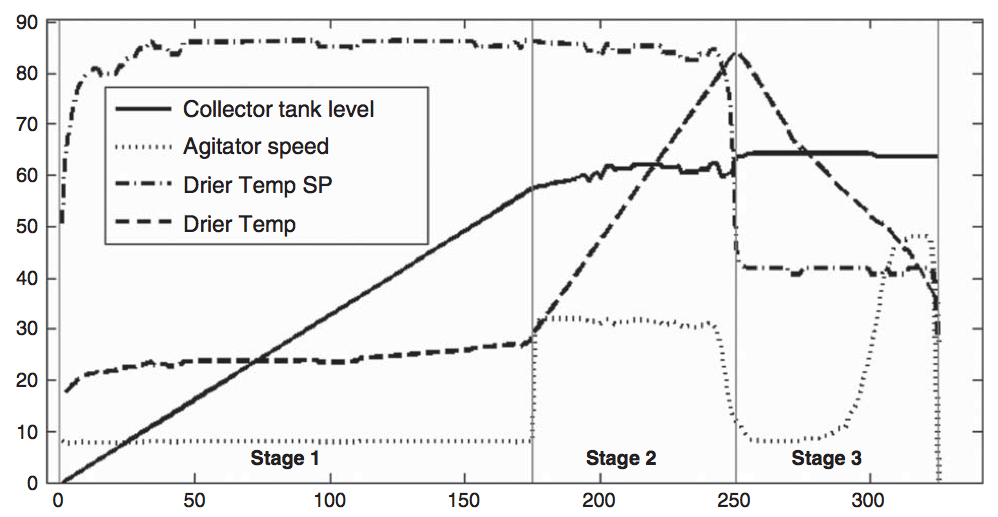
\includegraphics[width=\textwidth]{images/fmc/fmc-phases-4-trajectories.png}
	\end{center}
	
\end{frame}

\begin{frame}\frametitle{Class example: using feature-based models}

	\begin{itemize}
	
		\item	Features extracted:
	
	\end{itemize}

	\begin{center}
		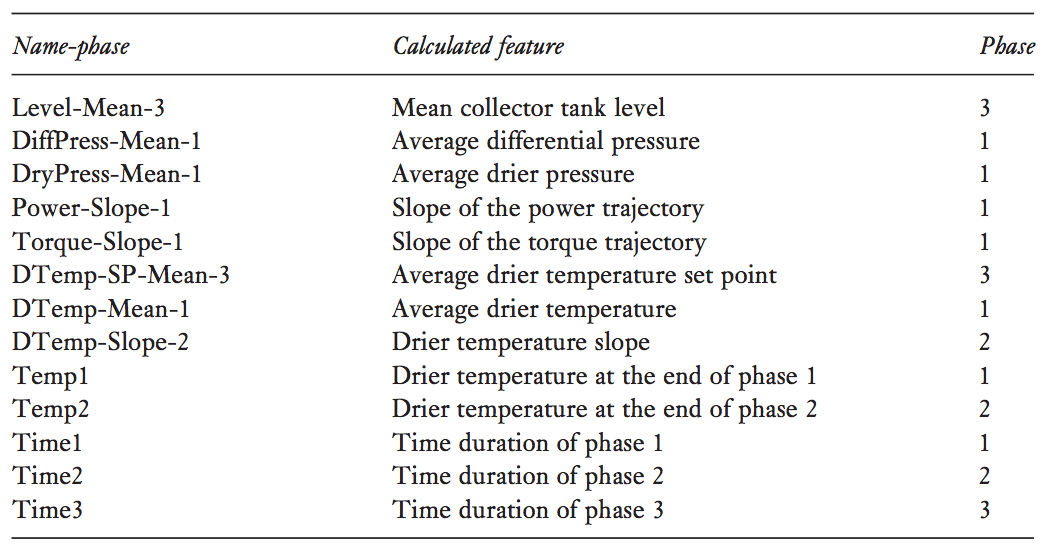
\includegraphics[width=\textwidth]{images/fmc/fmc-features-extracted.png}
	\end{center}
	
	\begin{itemize}
		\item	\( \mathbf{Z} \): recipe and compositions: 11 variables
		
		\item	\( \mathbf{X} \): the 13 extracted features
		
		\item	\( \mathbf{Y} \): 8 final quality variables
	\end{itemize}
	

\end{frame}

% 	\begin{center}
% 		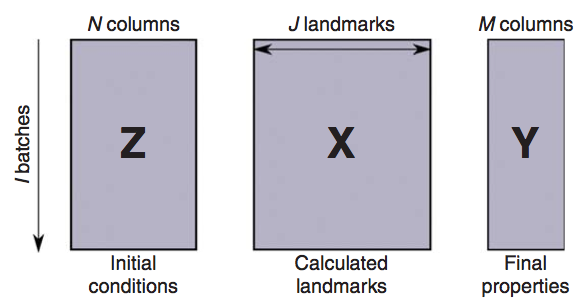
\includegraphics[width=\textwidth]{images/fmc/fmc-features-multiblock.png}
% 	\end{center}

\begin{frame}\frametitle{Class example: model results}
	
	\begin{itemize}
		\item	Score plot shows good clear separation between off-spec batches (red circles) and good product (black squares)
	\end{itemize}

	\begin{center}
		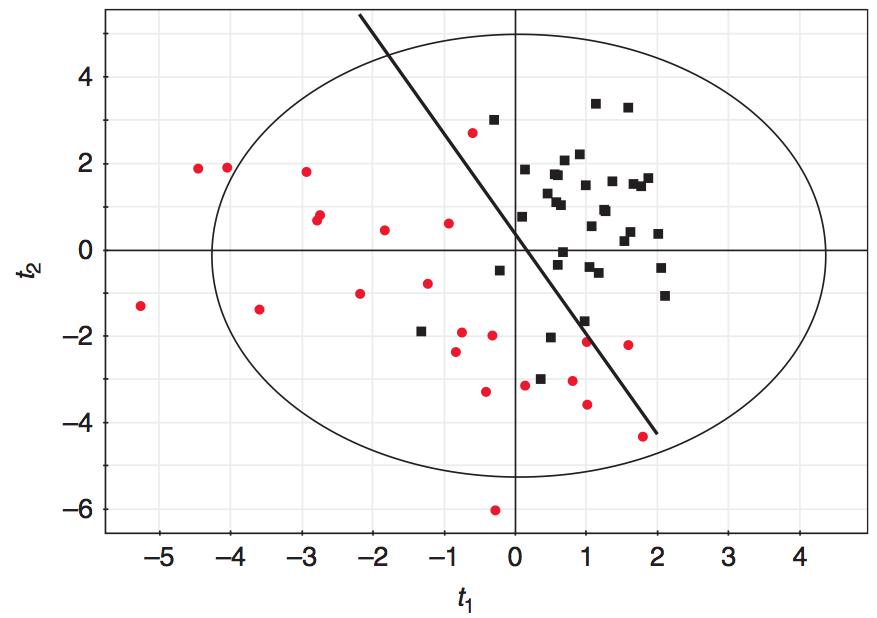
\includegraphics[width=0.9\textwidth]{images/fmc/fmc-score-plot-features.png}
	\end{center}
\end{frame}

\begin{frame}\frametitle{Class example: model results}
	
	\begin{itemize}
		\item	Loading plot for \( \mathbf{Z} \) and \( \mathbf{X} \) blocks
	\end{itemize}
	
	\begin{center}
		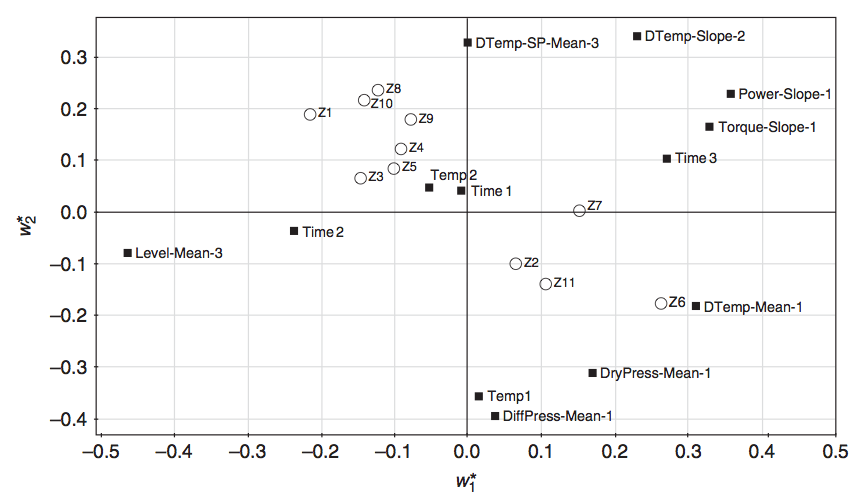
\includegraphics[width=\textwidth]{images/fmc/fmc-features-loading-plot.png}
	\end{center}
	
	\begin{itemize}
		\item	Good quality batches: operate at high \( t_1 \) and high \( t_2 \).
	\end{itemize}
	
\end{frame}

\begin{frame}\frametitle{Class example: model results}
	
	\begin{itemize}
		\item	VIP for \( \mathbf{Z} \) and \( \mathbf{X} \) blocks. Agrees with loadings.
	\end{itemize}
	
	\begin{center}
		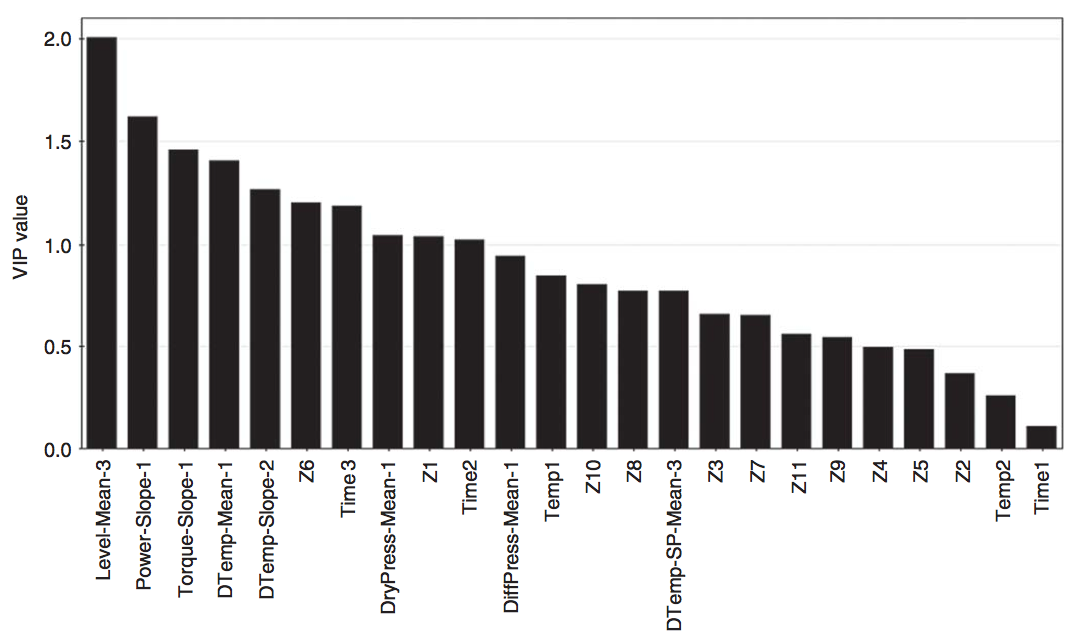
\includegraphics[width=\textwidth]{images/fmc/fmc-VIP-values-features.png}
	\end{center}
\end{frame}

\begin{frame}\frametitle{}

\end{frame}

% \begin{frame}\frametitle{Class example: what was learned?}
% 	
% 	To get good quality batches: operate at high \( t_1 \) and high \( t_2 \).  From loadings plot:
% 	
% 	\begin{itemize}
% 		\item	The plot shows that high rates of increase (slopes) of power, torque, and temperature in phase 1, as well as low solvent level in the collector tank in phase 3 (equivalent to low initial solvent in the wet cake) all relate to a good batch outcome
% 		% High t1: lower JTempSP slope:  But, JtempSlope is between -0.15 and -0.05, so a lower JTempSlope implies 
% 		% operation toward -0.15, ie temperature decreases more rapidly for the good batches. This might appear conflicting with the w*1 line plot, which shows that higher values of temperature SP lead to better batches.  How can a batch with a steeper decreasing slope have high value of temperature SP?  Well, the key insight is that temperature SP is always going to END at the same temperature value at the end of phase 2.  Having a steeper, more negative slope, implies that the batch must start at a higher temperature earlier in the batch.  This agrees exactly with the w*1 line plot.
% 	\end{itemize}
% 	
% 	Can be confirmed by looking at what trajectories for some good quality batches.
% 	
% 	\todo{Plot good quality batches}
% 	
% \end{frame}

